%% =====================================================================
%%  Hetero_MRI_Modelling_WRR -- draft 1
%%
%%  Evaporation-driven solute redistribution in a macroscopically
%%  heterogeneous porous media with a vertical textural interface:
%%  MRI observations and numerical analysis
%%
%%  Source of the text: ../Hetero_MRI_Modelling_WRR_draft1.docx
%%  LaTeX layout:      AGU/Water Resources Research template
%%                     (agujournal2019.cls, as used in
%%                     20DPNM/review-R2)
%%
%%  Build:  latexmk -pdf main.tex      (pdflatex + bibtex, apacite)
%%  Clean:  latexmk -c
%%
%%  Editorial helper macros:
%%    \authornote{...}  red in-line note that must be resolved before
%%                      submission (draft instructions, missing text)
%%    \figplaceholder{...}  framed placeholder for a figure whose
%%                      artwork is not yet available in pictures/
%% =====================================================================

\documentclass[final]{agujournal2019}

\usepackage{url}
\usepackage{lineno}
\usepackage{xcolor}
\usepackage{ifthen}
\usepackage{amsmath,amssymb}
\usepackage{graphicx}
\usepackage{booktabs}
\usepackage{array}

% Figures are stored in pictures/ next to this file.
\graphicspath{{pictures/}{./}}

\linenumbers
\draftfalse

\journalname{Water Resources Research}

% ---------------------------------------------------------------------
% Draft helpers
% ---------------------------------------------------------------------
% Red in-line note: draft instructions and text that is still missing.
% Remove every \authornote before submission.
\newcommand{\authornote}[1]{%
  \par\noindent\textcolor{red}{\small[\textbf{Author note:} #1]}\par}

% Framed placeholder for figures whose artwork is not yet in pictures/.
\newcommand{\figplaceholder}[1]{%
  \fbox{\begin{minipage}[c][5.2cm][c]{0.86\textwidth}%
    \centering\color{red}\small [Figure placeholder --- #1]%
  \end{minipage}}}

% Clickable repository link in pdfLaTeX (same definition as in the 20DPNM
% manuscript, so repository URLs stay clickable without changing the class's
% citation setup).
\newcommand{\repositoryurl}[1]{\leavevmode\pdfstartlink attr{/Border [0 0 0]}
  user{/Subtype /Link /A << /S /URI /URI (#1) >>}\url{#1}\pdfendlink}

% Shorthands for the two imaged nuclei.
\newcommand{\NaIso}{$^{23}$Na}
\newcommand{\HIso}{$^{1}$H}

\begin{document}

\title{Evaporation-driven solute redistribution in a macroscopically
heterogeneous porous media with a vertical textural interface:
MRI observations and numerical analysis}

%%%%%%%%%%%%%%%%%%%%%%%%%%%%%%%%%%%%%%%%%%%%%%%
%  AUTHORS AND AFFILIATIONS
%%%%%%%%%%%%%%%%%%%%%%%%%%%%%%%%%%%%%%%%%%%%%%%
\authors{M.~A. Chaudhry\affil{2}, Z.~Chen\affil{2}, A.~Pohlmeier\affil{1},
R.~Helmig\affil{2}, and J.~A.~Huisman\affil{1}}

\affiliation{1}{Agrosphere Institute (IBG~3), Forschungszentrum J\"ulich GmbH,
52428 J\"ulich, Germany.}
\affiliation{2}{Institute for Modeling Hydraulic and Environmental Systems
(IWS), University of Stuttgart, 70569 Stuttgart, Germany.}

\correspondingauthor{Zhixin Chen}{zhixin.chen@iws.uni-stuttgart.de}

%%%%%%%%%%%%%%%%%%%%%%%%%%%%%%%%%%%%%%%%%%%%%%%
%  KEY POINTS
%%%%%%%%%%%%%%%%%%%%%%%%%%%%%%%%%%%%%%%%%%%%%%%
%  Up to three points, each at most 140 characters, complete sentences,
%  no special characters or punctuation.
%  NOTE: draft points written from the abstract of draft1.docx; the
%  authors must confirm the wording before submission.
\begin{keypoints}
\raggedright
\item %%
      Time-resolved sodium MRI visualizes evaporation-driven salt redistribution across a vertical sand interface
\item %%
      Density-driven flow in the coarse sand and near-surface enrichment in the fine sand develop simultaneously
\item %%
      Diffusion across the interface reverses direction with depth and couples the two domains
\end{keypoints}

%%%%%%%%%%%%%%%%%%%%%%%%%%%%%%%%%%%%%%%%%%%%%%%
%  ABSTRACT
%%%%%%%%%%%%%%%%%%%%%%%%%%%%%%%%%%%%%%%%%%%%%%%
\begin{abstract}
Evaporation of saline water from saturated porous media produces near-surface
solute enrichment, however the resulting concentration distribution also depends
on transport within the pore space and across material interfaces. Previous
three-dimensional sodium magnetic resonance imaging (\NaIso-MRI) demonstrated that
dense saline solution can move downward through a sufficiently permeable sand,
whereas a less permeable material retains much of the accumulated salt near the
evaporating surface. In the current work, spatial and temporal redistribution of
dissolved NaCl was investigated in a hydraulically connected, continuously
supplied packing consisting of coarse F36 and fine W3 sand separated by a sharp
vertical interface using time-resolved \NaIso-MRI in combination with \HIso-MRI.
The F36 domain developed descending high-concentration structures within the
first hours, followed by substantial enrichment at depth, while the W3 domain
exhibited pronounced near-surface accumulation. The dissolved NaCl concentration
near the W3 surface approached the solubility limit between 96 and 108~h.
Spatial concentration differences across the interface changed direction with
depth; first-order Fickian calculations indicate diffusion from W3 into F36 near
the surface and from F36 into W3 deeper in the packing. The mean measured
evaporation rate was approximately 3.8~mm~d$^{-1}$, with little change in
near-surface water content. \HIso-MRI revealed initial signs of crust over the
W3 half towards the end of the experiment. These observations establish a
spatially coupled redistribution pattern that cannot be explained solely by the
behavior of either domain in isolation. Additionally, numerical simulations were
performed on an identical system using DuMu$^\mathrm{X}$ along with further
permeability contrasts and targeted salt transport process comparisons.
\authornote{Draft 1 ends the abstract with ``Details of simulations to be
added.'' The numerical sentence above is kept generic until the simulation
results are available (Sections~2.3 and 3.5).}
\end{abstract}

%%%%%%%%%%%%%%%%%%%%%%%%%%%%%%%%%%%%%%%%%%%%%%%
%  BODY TEXT
%%%%%%%%%%%%%%%%%%%%%%%%%%%%%%%%%%%%%%%%%%%%%%%
\newpage

\section{Introduction} \label{sec:introduction}

Evaporation from porous media such as soil supplied by shallow saline
groundwater can sustain upward liquid transport toward the atmosphere while
leaving dissolved salts behind in the pore solution
\cite{nachshon2011a,shokrikuehni2020}. As the water is removed, the
concentration of NaCl increases near the evaporating surface, lowering the water
activity of the remaining solution and potentially leading to salt
precipitation. This salinization process is known to cause significant soil
degradation and reductions in crop yield within arid and semi-arid regions
\cite{rodriguez1997,chaves2009}. The resulting distribution of salt depends on
water supply, surface saturation, the transport properties of the porous medium
and the location of the evaporation front
\cite{shimojima1996,nachshon2011b,shokrikuehni2020}. Under conditions where the
pore network remains hydraulically connected to a reservoir, salt accumulation
is not restricted to a drying front moving into the medium. Instead, the
near-surface concentration develops while liquid replenishment continues, making
internal transport mechanisms particularly important for predicting the
subsequent evolution of surface salinity.

The accumulation of salt increases the density of the pore solution and can
create a gravitationally unstable concentration boundary layer. The onset and
evolution of this instability have been investigated through analytical and
numerical studies of saline groundwater evaporation
\cite{wooding1997a,wooding1997b,bringedal2022}. Where intrinsic permeability is
sufficiently high, downward buoyant transport can compete with the upward solute
transport associated with evaporative supply and with diffusion or dispersion.
Direct experimental confirmation was provided by \citeA{chaudhry2026}, who used
three-dimensional \NaIso-MRI to compare homogeneous F36 and W3 sands. In the
higher-permeability F36 sand, descending saline plumes redistributed NaCl toward
the bottom of the sample, thereby limiting surface enrichment. The
lower-permeability W3 sand showed no corresponding instability and developed
strong concentration gradients confined largely to the near-surface region.
These findings establish the role of permeability-dependent downward transport in
homogeneous, saturated porous media, but do not establish how it interacts with
an adjacent material of contrasting texture.

A sharp textural interface introduces an additional pathway for solute
redistribution. When coarse and fine domains remain hydraulically connected,
differences in pore pressure, water supply, and evolving salt concentration can
produce lateral fluxes of liquid and dissolved solute
\cite{lehmann2009,shahraeeni2010}. Previous investigations of evaporation from
heterogeneous porous media have demonstrated that material configuration
influences surface wetness, evaporative fluxes and precipitation patterns
\cite{nachshon2011b,shokrikuehni2020}. However, an unresolved question for
continuously saturated systems is whether downward redistribution in a highly
permeable domain can alter salt storage and surface enrichment in a neighboring,
low-permeability domain. In particular, local concentration gradients may drive
diffusion in opposite directions at different depths, while changes in hydraulic
flow may contribute additional interdomain transport. Observing a concentration
contrast across the interface, on its own, does not determine the net transport
budget or separate advective and diffusive contributions.

While the previously mentioned experimental studies establish the importance of
hydraulic coupling and heterogeneity, the individual contributions of advective
and diffusive transport to net dissolved-salt exchange across an interface remain
insufficiently quantified. Extending current numerical investigations
\cite{wooding1997a,wooding1997b,bringedal2022,lasser2023,chen2026} to
hydraulically connected porous media with contrasting permeabilities, while
systematically varying permeability contrasts and evaporative conditions, could
therefore provide a more detailed understanding of interfacial solute transport.
In particular, quantifying the spatially and temporally varying advective and
diffusive contributions, together with their combined net flux across the
interface, is essential for establishing the extent to which interdomain solute
exchange modifies near-surface enrichment and the overall redistribution of salt
during evaporation.

This study investigates evaporation-driven NaCl redistribution in a
heterogeneous packing of relatively coarser F36 and fine W3 sand coupled across a
vertical interface. The objectives are to (i) characterize the three-dimensional
evolution of dissolved-salt concentrations within each domain; (ii) identify the
observed interfacial concentration gradients and determine the processes
responsible for interdomain exchange; and (iii) assess how hydraulic connection
modifies surface enrichment compared with the corresponding disconnected
configurations. The experimental analysis combines time-resolved \NaIso-MRI,
\HIso-MRI and evaporation measurements. The accompanying numerical investigation
is designed to quantify conservative interfacial fluxes and evaluate the
contribution of density-driven flow through matched process comparisons. The
experimental measurements and the numerical analysis will thus be used together
to distinguish directly observed redistribution from modeled transport
mechanisms.

\section{Materials and methods} \label{sec:methods}

\subsection{Porous materials and experimental configuration}
\label{sec:materials}

Two quartz sands with contrasting texture and intrinsic permeability were
selected: F36 and W3, both supplied by Quarzwerke Frechen GmbH (Frechen,
Germany). Their hydraulic properties were determined in accordance with methods
elaborated in \citeA{chaudhry2026} by fitting the Brooks--Corey model to measured
water-retention data and calculating intrinsic permeability from saturated
falling-head conductivity measurements. The resulting intrinsic permeabilities
were $7.83\times10^{-12}$~m$^2$ for F36 and $3.2\times10^{-14}$~m$^2$ for W3.
The material properties relevant to the present experiments are summarized in
Table~\ref{tab:properties}.

\begin{table}[t]
\centering
\caption{Properties of the two materials used for the evaporation experiments.
Particle size ranges were provided by the supplier (Quarzwerke Frechen). The
parameters of the Brooks--Corey model were obtained by fitting to measured water
retention data.}
\label{tab:properties}
\begin{tabular}{lcc}
\toprule
 & F36 & W3 \\
\midrule
Average particle size ($\mu$m)              & 160 & 90 \\
Particle size range ($\mu$m)                & 90--355 & 2--400 \\
Type (USDA)                                  & medium sand & very fine sand \\
Intrinsic permeability (m$^2$)              & $7.83\times10^{-12}$ & $3.2\times10^{-14}$ \\
Brooks--Corey saturated water content $\theta_{\mathrm{sat}}$ (cm$^3$~cm$^{-3}$)  & 0.39 & 0.31 \\
Brooks--Corey residual water content $\theta_{\mathrm{res}}$ (cm$^3$~cm$^{-3}$)   & 0.02 & 0.08 \\
Entry pressure $p_b$ (Pa)                    & $4.69\times10^{3}$ & $1.12\times10^{4}$ \\
Brooks--Corey parameter $\lambda_{\mathrm{BC}}$ & 5.04 & 0.384 \\
\bottomrule
\end{tabular}
\end{table}

The heterogeneous sample was prepared in a non-metallic polymethylmethacrylate
(PMMA) holder with an inner diameter of 5~cm and a packing height of 4~cm
(Figure~\ref{fig:setup}). A 0.45-cm-thick porous filter plate (P3, Robu, Hattert,
Germany) was installed at the bottom. A temporary $5\times5\times0.6$~cm PMMA
partition divided the sample cavity into two equal semicircular domains, which
were filled separately with dry F36 and W3 sand. The central partition was then
removed slowly while the holder was gently tapped to maintain a sharp vertical
material interface. Dry packing was selected because removing the partition after
wet packing caused deformation of the interface and introduced air or water
pockets. The prepared sample was saturated from below with 1~mol~L$^{-1}$ NaCl
(Sigma-Aldrich Chemie GmbH, Taufkirchen, Germany) solution while evaporation
from its upper surface was prevented with a Parafilm covering.

An external reservoir containing the same 1~mol~L$^{-1}$ NaCl solution was
connected to the bottom inlet. Its water level was adjusted to 2~cm below the
sample surface, and the system was allowed to equilibrate for 2~h. The initial
volumetric water content of the packed sample, obtained from the solution mass
retained after saturation, was calculated to be 0.38. With $m_{\mathrm{sol}}$
denoting the retained solution mass, $\rho_{\mathrm{sol}}$ its density and
$V_{\mathrm{pa}}$ the bulk packing volume, the volumetric content was obtained as
$\theta = m_{\mathrm{sol}}/(\rho_{\mathrm{sol}}V_{\mathrm{pa}})$. Continuous
hydraulic contact with the reservoir was maintained throughout evaporation
(wicking). The 1~mol~L$^{-1}$ NaCl concentration was used as it was found to be
suitable for providing a high enough concentration range for downwards
density-driven flow.

The sample holder featured a wider internal diameter that fit into the \NaIso/\HIso{}
66~mm wide probe head (Bruker Mini SWB~90 imaging probe DR) of the MRI scanner
(Bruker super wide bore scanner at $B_0 = 4.7$~T). The bottom inlet was opened
and the dry-gas diffuser was switched on to generate a turbulent stream of
N$_2$ gas at 60~dm$^3$~h$^{-1}$, thus initiating evaporation. Ambient laboratory
conditions were monitored using a multi-purpose probe (FHAD 46-C2, ALMEMO
D06, Ahlborn, Holzkirchen, Germany). The mean temperature and ambient humidity
were relatively stable at $20 \pm 2\,^\circ$C and 40\,\% $\pm$ 2.5\,\%. The
evaporation rate $E_{\mathrm{rate}}$ was determined from the mass change of the
reservoir recorded hourly with a balance (accuracy $\pm$0.01~g, EX2202, Ohaus
Corporation, Parsippany, USA) using:
\begin{equation}
E_{\mathrm{rate}} = \frac{\Delta m}{\rho_{\mathrm{sol}}\,A_{\mathrm{evap}}\,t_{\mathrm{diff}}},
\label{eq:evaporation-rate}
\end{equation}
where $\Delta m = m_1 - m_2$ is the mass difference during the time interval
$t_{\mathrm{diff}} = t_1 - t_2$, and $A_{\mathrm{evap}}$ is the evaporative area.

\begin{figure}[t]
\centering
\begin{minipage}[b]{0.47\textwidth}
  \centering
  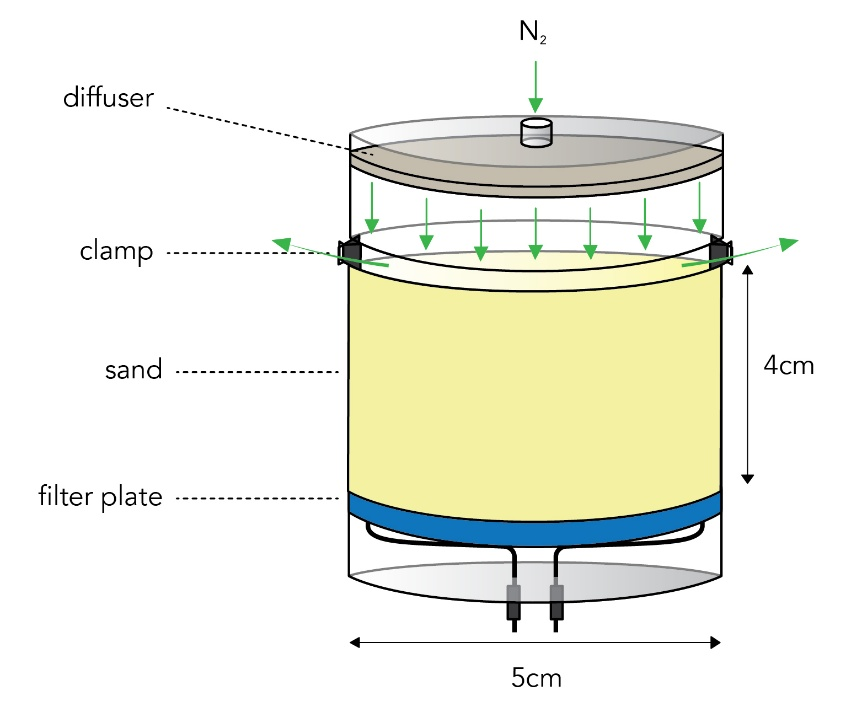
\includegraphics[width=\linewidth]{pictures/fig01a_holder.jpeg}\\
  (a)
\end{minipage}\hfill
\begin{minipage}[b]{0.47\textwidth}
  \centering
  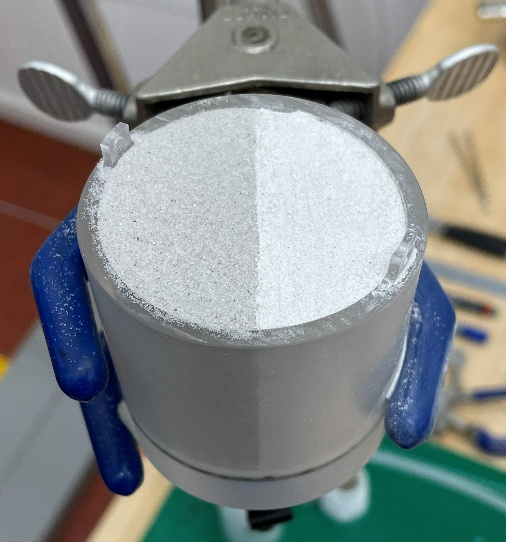
\includegraphics[width=\linewidth]{pictures/fig01b_packing.png}\\
  (b)
\end{minipage}
\caption{(a) Adapted sample holder design used for performing evaporation
experiments on heterogeneous porous media within the MRI. (b) Sample with a
vertical interface of the packed sand in the sample holder with the gas
distributor removed.}
\label{fig:setup}
\end{figure}

\subsection{MRI acquisition and calibration} \label{sec:mri}

The experiment was conducted using a Bruker super wide bore scanner with a
$B_0$ field strength of 4.7~T. The 3D orthogonal gradient/shimming system was
capable of delivering a maximum gradient strength of 700~mT~m$^{-1}$. The
scanner was run using an Avance~III console and controlled by Paravision
software (version~6, Bruker Microimaging, Ettlingen, Germany). Due to the
faster $T_2$ relaxation of brine in the W3 sample \cite{chaudhry2026}, the
acquisition parameters were shifted to accommodate this
(Table~\ref{tab:imaging}). Due to the early development of instabilities in F36,
it was essential to keep the scan time for \NaIso{} imaging short. The experiment
started with an initial \NaIso{} scan before the N$_2$ gas stream was turned on.

\begin{table}[t]
\centering
\caption{Key parameters of the imaging protocols adopted for \HIso{} and
\NaIso{} MRI during evaporation from the heterogeneous F36 and W3 sample. The
native Bruker protocols to which adjustments were made are 3D single echo
(3DSE) and multi-slice multi-echo (MSME).}
\label{tab:imaging}
\begin{tabular}{lcc}
\toprule
 & \NaIso{} imaging & \HIso{} imaging \\
\midrule
Pulse sequence          & 3DSE & MSME \\
$t_R$ (ms)              & 300 & 3000 \\
$t_E$ (ms)              & 4.6 & 4 \\
Slices                  & 1 & 40 \\
Slice thickness (mm)    & 55 & 1 \\
Number of averages      & 4 & 4 \\
Scan time (min)         & 32 & 51 \\
Matrix size             & $64\times40\times40$ & $256\times256\times1$ \\
Resolution (mm)         & $1\times1.375\times1.375$ & $0.25\times0.25\times0.25$ \\
Bandwidth (kHz)         & 50 & 150 \\
\bottomrule
\end{tabular}
\end{table}

The scan intervals for the heterogeneous sample were kept shorter in the initial
stages of the experiment. After the initial scan, imaging was performed in the
following sequence: $8\times30$~min, $2\times60$~min, $3\times120$~min, and
$27\times360$~min. The total duration of the experiment was 174~hours.

\HIso{} scans were periodically performed to ensure that the sample remained
fully saturated throughout the evaporation experiment. The sample holder
dimensions did not allow the use of a marker tube for calibration. Therefore,
the known initial volumetric water content $\theta$ of the sample (0.38) was used
for calibration instead. The subsequent scans were then normalized against this
scan to identify any changes in volumetric water content.

Na concentration profiles were determined using a calibration approach where F36
and W3 packings in the sample holder were saturated with known concentrations of
0, 1, 2, 3, 4 and 5~mol~L$^{-1}$ solution and scanned using the imaging
protocols shown in Table~\ref{tab:imaging}. The average voxel intensity of the
calibration samples was plotted against the Na volume concentration using the
relationship \cite{perelman2020}:
\begin{equation}
c_{\mathrm{Na,vol}} = \frac{n_{\mathrm{Na}}}{V_{\mathrm{bulk}}}
= c_{\mathrm{Na,sol}}\,\theta_{\mathrm{vol}},
\label{eq:calibration}
\end{equation}
where $n_{\mathrm{Na}}$ is the number of moles of Na, $V_{\mathrm{bulk}}$ is the
bulk volume, $c_{\mathrm{Na,sol}}$ is the solution concentration and
$\theta_{\mathrm{vol}}$ is the volumetric water content. It was then fitted with
a linear function for F36 and a polynomial function for W3.

Data processing of the raw MRI data involved several steps. First, the acquired
k-space data was reconstructed into spatial domain images through inverse Fourier
transformation using the Paravision software package (version~6, Bruker
Microimaging, Ettlingen, Germany). The resulting images were then further
processed with ImageJ (version~1.53t, National Institutes of Health (NIH),
Bethesda, USA). All scans were equally scaled using the brightness/contrast
function and then set to a standardized brightness range within the used color
table for enhanced visualization. To reduce noise, a 1.5~pixel median filter was
applied. Additionally, transparent 3D illustrations were generated using the
volume viewer plugin to highlight internal features of the samples. During data
acquisition, a spike artifact was detected in the sample space, which was removed
to the extent possible in the 3D visualization by filtering out high voxel values
in this region.

\subsection{Numerical model and boundary conditions} \label{sec:numerical-model}

\authornote{Section still to be written. The draft states that numerical
simulations were performed on an identical system using DuMu$^\mathrm{X}$,
including further permeability contrasts and targeted salt transport process
comparisons. Planned content: governing equations and constitutive relations
(NaCl mass fraction, density, viscosity, water activity), computational domain
and discretisation, initial and boundary conditions, and the connected versus
isolated interface configurations used for the process comparison.}

\subsection{Quantities used for model comparison} \label{sec:quantities}

\authornote{Section still to be written. Planned content: definitions of the
integrated Na mass in each half, conservative interfacial flux (advective and
diffusive), surface enrichment, and the error measures used to compare simulated
and measured concentration profiles.}

\subsection{Process comparisons and numerical verification} \label{sec:process-comparison}

\authornote{Section still to be written. Planned content: the paired
connected--disconnected simulations, the permeability-contrast series, and the
verification of the numerical implementation (e.g., mass balance and grid
convergence).}

\subsection{Dimensionless parameters and regime classification} \label{sec:regime}

\authornote{Section still to be written. Planned content: the definition of the
boundary-layer Rayleigh number $R_\delta$ used in Section~\ref{sec:profiles} and
the dimensionless parameters that organize the connected--isolated comparison
into regimes.}

\section{Results and discussion} \label{sec:results}

\subsection{Evaporation dynamics of the heterogeneous porous media}
\label{sec:evaporation}

The cumulative water loss over time for the heterogeneous sand packing
containing F36 and W3 is presented in Figure~\ref{fig:evaporation}a. The
evaporation rate as a function of time is presented in
Figure~\ref{fig:evaporation}b along with the observed volumetric water content
for the top 2~mm of the sample at three distinct times. The water content in the
top 2~mm remained constant despite ongoing evaporation, thus ensuring saturation
throughout the duration of the experiment. The flow rate for dry nitrogen gas was
the same as in \citeA{chaudhry2026} but the surface area of the sample
significantly increased from 7.0~cm$^2$ to 19.6~cm$^2$. Therefore, the mean
evaporation rate was lower. The initial evaporation rate was approximately
6~mm~d$^{-1}$ and reduced to 3.8~mm~d$^{-1}$ in the first 24~hours. The average
evaporation rate for the experimental duration of 174~hours was
3.8~mm~d$^{-1}$. A sharp decrease in evaporation rate is seen for the
heterogeneous packing in the first 4~hours which then becomes more gradual with
time. This is attributed to a thin water film and minor settling during
installation of the sample in the MRI, as well as stronger near-surface solute
enrichment for W3. Beyond this sharp initial decrease, the evaporation rate
decreased from 4.0~mm~d$^{-1}$ to 3.2~mm~d$^{-1}$ after the first four hours.
This decrease is much smaller than the decrease observed for pure W3, but higher
than the near constant rate observed for pure F36 \cite{chaudhry2026}. As
expected, the evaporation dynamics of the heterogeneous medium falls between the
behavior of the individual materials.

\begin{figure}[t]
\centering
\figplaceholder{cumulative water loss (a) and evaporation rate plus top-2-mm
water content (b); artwork not included in draft1.docx}
\caption{(a) Cumulative mass loss of water during the evaporation experiment for
the heterogeneous F36 and W3 packing with a vertical interface under wicking
conditions. (b) Evaporation rate for the heterogeneous F36 and W3 packing and the
volumetric water content $\theta$ in the top 2~mm of the sample at 0~h, 24~h and
174~h from the start of the experiment (right ordinate).}
\label{fig:evaporation}
\end{figure}

\subsection{Calibration of $^{23}$Na-MRI for heterogeneous sand packing}
\label{sec:calibration}

To determine Na concentration profiles, calibration relationships were developed
for the sample holder and acquisition protocol used in this investigation. As
predicted, a linear calibration relationship was obtained for F36, which reflects
the bulk-like relaxation behavior of Na in F36. A slightly non-linear relation
was obtained for W3, which could be well described by a polynomial fit. The shape
of this new calibration relationship deviates from the earlier calibration
reported by \citeA{chaudhry2026}, which was obtained using a slightly longer echo
time $t_E$ of 5.1~ms. By adopting an imaging protocol for a shorter total scan
time and a long enough $t_E$ to capture bulk relaxation in F36, the slope of the
signal response $S(r)$ apparently decreased for higher solute concentrations in
W3. For \citeA{chaudhry2026} the slope of $S(r)$ increased with increasing
concentration, which was attributed to stronger shielding of the surface charge
at increased ionic strengths \cite{rijniers2004}. However, this effect was much
lower for the current acquisition protocol. Further investigation is required to
fully understand the dependence of the measured signal on ionic strength and
material properties. Consequently, the present calibration approach should be
regarded as an empirical and practical method for obtaining quantitative
estimates of Na concentration in porous media.

The relatively low SNR for \NaIso-MRI led to variations in voxel signal intensity
for the heterogeneous sample. The obtained calibration relationships can be used
to re-calculate the known Na concentrations of the calibration samples. Assuming
that all observed variation within the calibration samples is due to the low SNR,
the standard deviation of the concentration in the total voxel area of each
sample (after filtering) can be used as an estimate of uncertainty in estimated
concentration (Figure~\ref{fig:calibration}). The obtained standard deviations
for the solution concentrations in the F36 calibration series (i.e.\ 0, 1, 2, 3,
4 and 5~mol~L$^{-1}$) were 0.11, 0.26, 0.35, 0.42, 0.51 and 0.63, respectively.
Thus, the mean relative error in the concentration estimates is $\sim$14\,\%,
and is higher for the lowest concentrations. The standard deviations of the
concentration estimates obtained for W3 were 0.13, 0.28, 0.29, 0.54, 0.67 and
0.63 concerning the calibration samples. This indicates a similar relative error
for higher concentrations ($\sim$15\,\%) and higher relative errors for the lower
concentrations. The slight increase in relative error compared to the results in
\citeA{chaudhry2026} can be attributed to the more challenging sample
preparation when the sample is larger. The change in packing method to dry
packing with subsequent water saturation may also have led to minor air
entrapment. It is important to mention that this approach to error
characterization is a worst-case scenario since all actual heterogeneity in
packing density is considered within the error estimation.

\begin{figure}[t]
\centering
\figplaceholder{calibration curves for F36 and W3 (time-averaged voxel
intensity versus Na volume concentration); artwork not included in
draft1.docx}
\caption{Calibration results for F36 and W3 using an identical imaging protocol
where average voxel signal intensity ($S_r$) is related to the volume
concentration of sodium $c_{\mathrm{Na,vol}}$ obtained with
Equation~\ref{eq:calibration}. The dotted lines are a linear and a second-order
polynomial fit with the parameters shown in the plot. Error bars represent one
standard deviation of voxel intensity after the use of a 1.5~pixel median
filter.}
\label{fig:calibration}
\end{figure}

\subsection{Na enrichment and redistribution during evaporation}
\label{sec:enrichment}

Figure~\ref{fig:na-first8h} shows the spatial and temporal development of the Na
concentration for the heterogeneous F36/W3 sand packing during the first
8~hours. The time gap between acquisitions was kept short here to capture
instability formation and downward density-driven flow. During this initial
stage of evaporation, a minor enrichment of sodium concentration was observed
near the surface of W3 and F36. This enrichment was more patchy for the F36
surface, whereas a more uniform enrichment was observed for W3. Although a sharp
and distinct finger could not be observed initially in F36, a high concentration
instability patch was observed near the top right of the F36 surface
(Figure~\ref{fig:na-first8h}, red arrow at $T=2$~h). Between 3~h and 4~h, a
gradual descent of this region with higher concentration was observed. Another
high concentration zone in the center of the F36 packing also highlights a site
for potential finger formation (Figure~\ref{fig:na-first8h}b, red arrow at
$T=8$~h). In contrast to F36, W3 showed only localized near-surface enrichment.
This behavior was anticipated due to the two orders of magnitude difference in
intrinsic permeability between the two porous media, thus promoting divergent
enrichment dynamics from the onset of evaporation.

\begin{figure}[t]
\centering
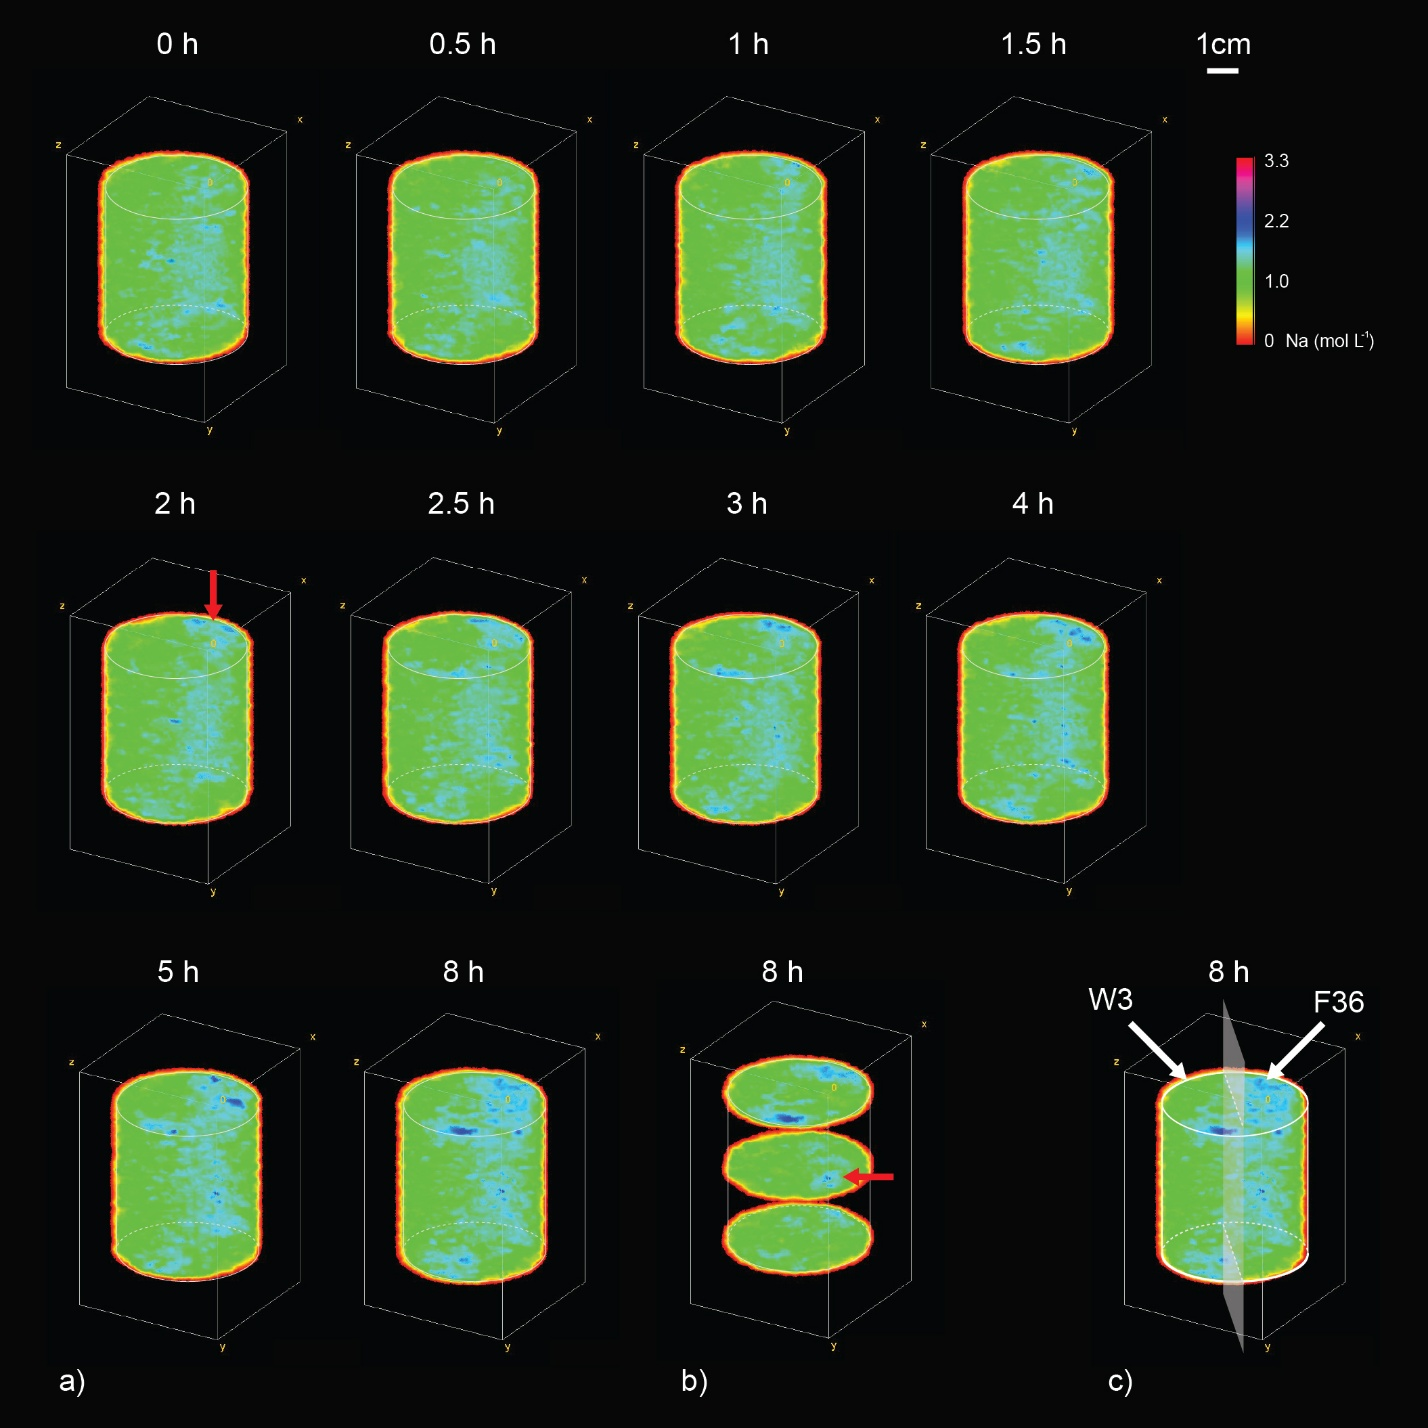
\includegraphics[width=0.92\textwidth]{pictures/fig04_na_first8h.jpeg}
\caption{(a) 3D voxel view of \NaIso-MRI imaging results as Na concentration for
the first 8~hours of evaporation. (b) Top, center and bottom slabs (3.9~mm
thickness) at 8~h that indicate instabilities. (c) 3D view of a \NaIso-MRI
imaging result highlighting W3 and F36 halves connected at a vertical interface.
Red arrows mark regions of interest; white arrows and the plane mark the W3 and
F36 halves and the vertical interface, respectively.}
\label{fig:na-first8h}
\end{figure}

Figure~\ref{fig:na-full}a shows the spatial and temporal development of the Na
concentration for the heterogeneous F36/W3 sand packing during the entire length
of the experiment. As expected, there is a strong surface enrichment of Na in the
W3 half of the sample. The Na concentration value reaches the solubility limit
between 96 and 108~hours, and enrichment is mostly confined to the upper half of
the W3 material. In contrast, F36 shows a relatively even enrichment throughout
the sample depth due to downward density-driven flow. The cross-sectional images
provided in Figure~\ref{fig:na-full}b indicate the positions of the fingers that
redistributed Na to the bottom of the packing. The minor fingers initially
visible in Figure~\ref{fig:na-full}a have evolved into mature convective plume
structures. The fingers are primarily located near the sample holder wall. The
concentration within a cross-sectional slice in the center of the sample ranges
between 1~mol~L$^{-1}$ to upwards of 4~mol~L$^{-1}$
(Figure~\ref{fig:na-full}b). This range is considerably higher than the estimated
relative error of approximately 15\,\% in concentration for the new imaging
protocol. This further strengthens confidence in the use of \NaIso-MRI for imaging
unstable flows.

\begin{figure}[t]
\centering
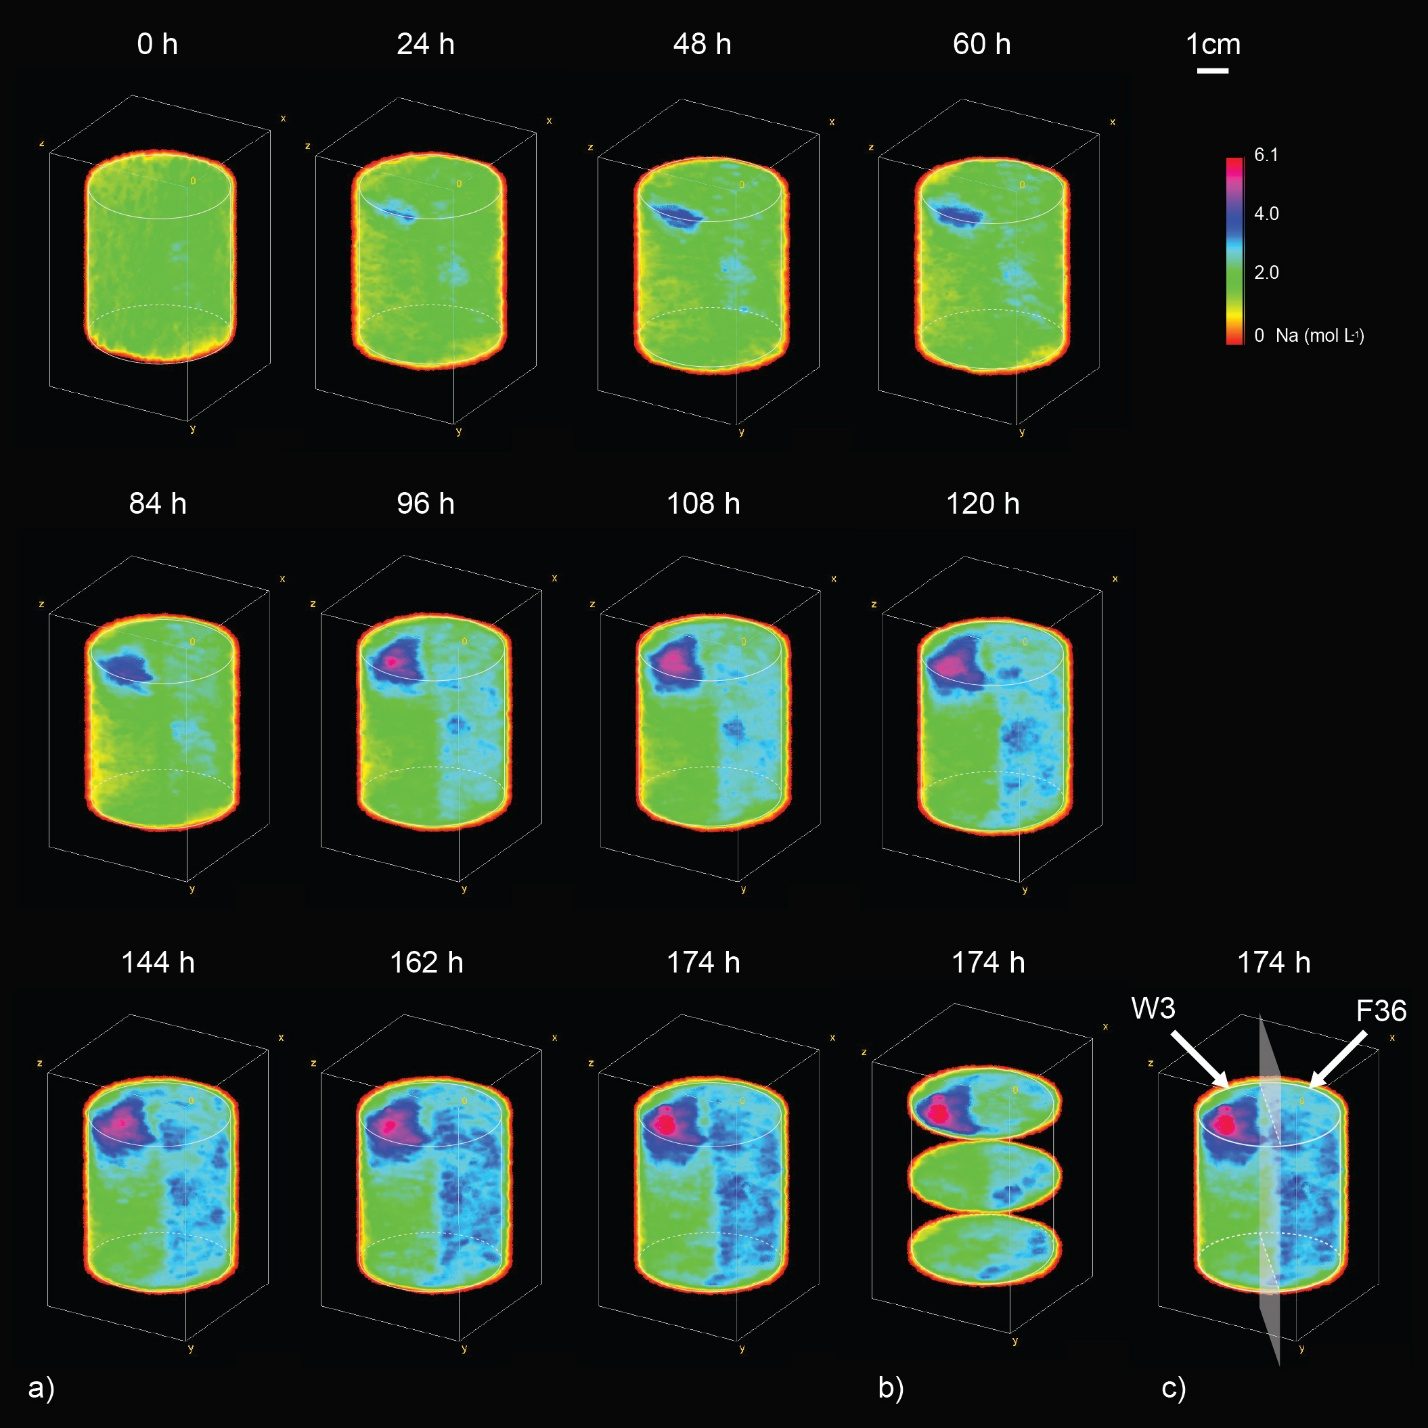
\includegraphics[width=0.92\textwidth]{pictures/fig05_na_full.jpeg}
\caption{(a) 3D view of \NaIso-MRI imaging results as Na concentration for the
entire duration of the evaporation experiment. (b) Top, center and bottom slabs
(3.9~mm thickness) at 174~h that indicate instabilities. (c) 3D view of a
\NaIso-MRI imaging result highlighting W3 and F36 halves connected at a vertical
interface.}
\label{fig:na-full}
\end{figure}

Strong downward density-driven flow was observed in the F36 half. The lack of a
central or sharply defined density instability may be attributed to the new
packing geometry where each material only takes up 50\,\% of the sample volume.
The larger ratio of sand volume to wall contact area of the F36 half in the
current experiment may have caused instability formation near the sample wall,
further strengthening with time. The finger observed by \citeA{chaudhry2026} in
homogeneous F36 packing and in the numerical simulation for the identical system
also advanced towards the sample holder wall with time. The diameter of the
current sand packing is constrained by the probe head diameter of the used MRI
system. Future research could use a wider bore MRI to image unstable flows in
larger samples that are less affected by wall effects to capture instabilities in
heterogeneous sand packings with more detail.

The duration of this experiment was kept long enough to generate indications of
salt crust on the W3 half of the sample. Figure~\ref{fig:crust} shows the 1~mm
thick top slice of the sand packing using Na imaging alongside the corresponding
cross-sectional \HIso{} imaging results that provide the volumetric water content
in the top 10~mm of the packing. Due to evaporation, a strong enrichment of Na at
the sample surface is seen on the W3 half. Although \NaIso-MRI cannot capture
precipitated NaCl, the associated \HIso{} imaging results indicate the presence
of moisture inside an evolving NaCl crust that creates a new porous media on top
of the original sample surface \cite{wieboldt2023}. No salt crusts and water
inside potential salt crusts are observed for the F36 half. The position of the
developing salt crust deduced from \HIso{} imaging matches the position where Na
concentration is highest in the Na imaging.

\begin{figure}[t]
\centering
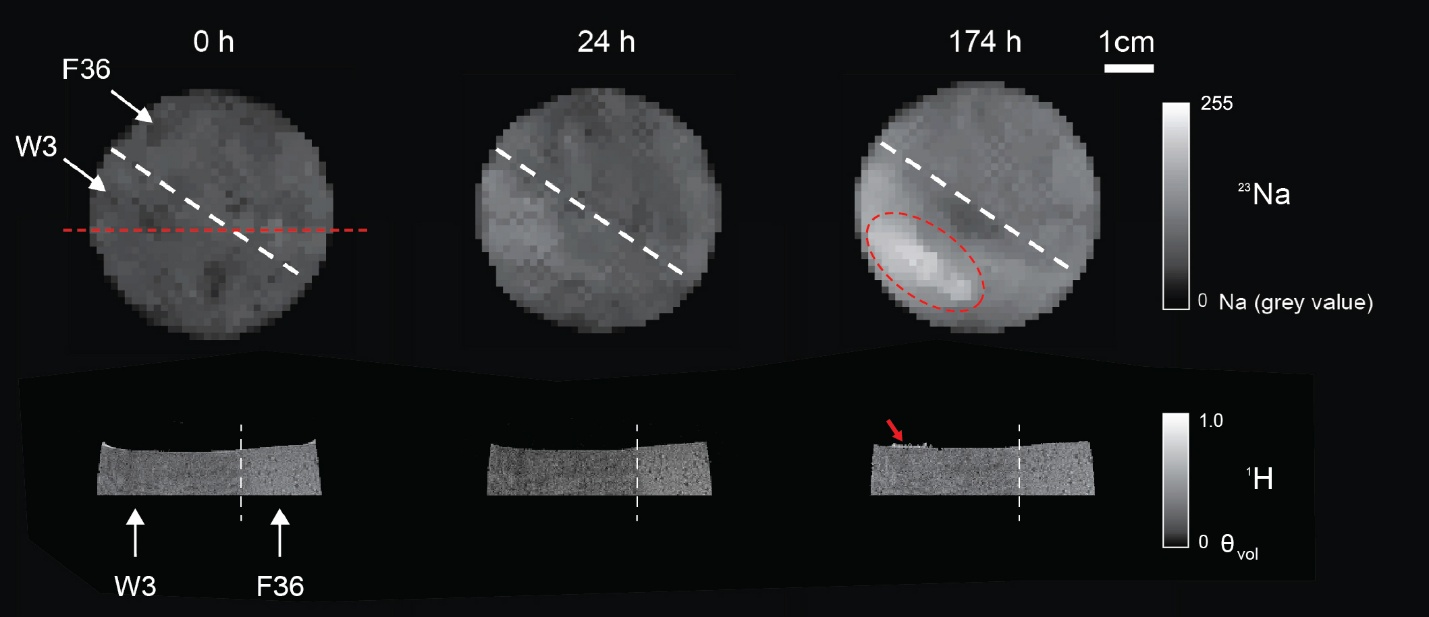
\includegraphics[width=0.95\textwidth]{pictures/fig06_h1_top.jpeg}
\caption{Cross-sectional view of the top 10~mm captured by \HIso-MRI at time 0~h,
24~h and 174~h (bottom) alongside the corresponding top view of the heterogeneous
sand packing using \NaIso-MRI (top). Brightness of the voxels corresponds to the
volume concentration of the target nuclei. The dashed white line in the imaging
indicates the interface between the two media. The dashed straight red line
indicates the position of the cross-sectional view extracted from \HIso-MRI. The
red arrow and the oval-shaped red line indicate regions of interest for salt
precipitation.}
\label{fig:crust}
\end{figure}

These results highlight the importance of distinguishing evaporation from fully
saturated and partially saturated samples. In fully saturated conditions, air
entry does not occur and both coarse and fine domains remain hydraulically
connected to the evaporating surface. The observation that salt precipitation may
initiate in the fine textured domain under such conditions therefore provides an
important first indication that precipitation patterns can differ from those
observed in partially saturated systems. For example, \citeA{shokrikuehni2020}
showed that evaporation from a partially saturated heterogeneous system leads to
earlier salt crust formation on the partially saturated coarse sand. This is not
consistent with the results seen in Figure~\ref{fig:crust}, where the opposite is
observed for the fully saturated sample in this experiment. This apparent
contradiction is due to the larger mass and solute fluxes from the fewer active
pores at the surface of a partially saturated system. These higher fluxes
eventually lead to fast solute enrichment and strong crust production
\cite{norouzirad2013,shokri2014,shokrikuehni2020}.

\subsection{Salt concentration profiles and implications for evaporation}
\label{sec:profiles}

A comparison of the amount of Na recovered with \NaIso-MRI and the amount of Na
present in the column based on the initial concentration and the mass loss data
of the external reservoir is presented in Figure~\ref{fig:profiles}a. Initially,
the difference in mass is low. However, the deviations in mass rise and reach up
to 23\,\% with time after the start of the evaporation due to underestimation of
the Na concentration by \NaIso-MRI. With time, the difference in mass reduced
again to an underestimation of 10--15\,\% in the final stages of the evaporation
experiment. This increased error in \NaIso-MRI compared to that observed in
\citeA{chaudhry2026} may be due to the following reasons. Firstly, the new
imaging protocol used a coarser resolution and less averaging to achieve shorter
acquisition time in an attempt to capture the development of instabilities in the
heterogeneous packing. The reduced spatial resolution resulted in larger partial
volume effects and the reduced averaging decreased the signal-to-noise ratio
(SNR) (i.e.\ SNR improves with the square root of the number of averages).
Secondly, the results presented in Figure~\ref{fig:crust} indicate the presence
of a solid NaCl crust at the sample surface that remains undetected by
\NaIso-MRI, which also adds to the underestimation of the total Na content within
the column since precipitated salt is not detected. Finally, the higher error may
also be related to supersaturation due to delayed nucleation, since such high
concentration values were not considered during calibration. Nevertheless,
recovery of the mass with \NaIso-MRI is considered to be adequate for
investigating solute enrichment and redistribution in heterogeneous samples.

Depth profiles of Na concentration throughout the total cross-section, W3 half,
and F36 half are presented in Figure~\ref{fig:profiles}b--d, respectively. The
average Na concentration profiles for the entire sample
(Figure~\ref{fig:profiles}b) visually seem to correspond with the average of the
homogeneous F36 and W3 reported by \citeA{chaudhry2026}. The enrichment is
strongest with large gradients near the surface, but redistribution is also
evident throughout the entire sample. The solute distribution in the W3 half of
the sample (Figure~\ref{fig:profiles}c) shows the expected near-surface enrichment
for this material. The low permeability of the W3 sand hampers the formation of
instabilities and downward solute transport. As strong enrichment takes place in
W3, nucleation is hypothesized to have initiated between 96 and 108~hours, and
the ensuing crystal growth process acts as a sink, drawing ions from its
surroundings \cite{scherer2004}. It is interesting to note the increase in
concentration near the bottom of the W3 sample, which is attributed to lateral
transport from the adjacent F36 material.

The concentration profiles for the F36 half (Figure~\ref{fig:profiles}d) clearly
show that solute is convectively transported downwards due to its higher
permeability during evaporation. This density-driven downward distribution leads
to concentration profiles that show a uniform increase in concentration, even in
the lowest most depths. Differences in solute concentration between the W3 and
F36 half lead to local concentration gradients across the interface, and Na
transport through solute diffusion should thus be anticipated along the length of
the sample.

\begin{figure}[t]
\centering
\figplaceholder{(a) Na mass recovered by \NaIso-MRI versus Na mass from the
reservoir mass loss and (b--d) depth profiles for the total sample, W3 half and
F36 half; artwork not included in draft1.docx}
\caption{(a) The calculated amount of Na from \NaIso-MRI against the total amount
of Na in the column calculated from the initial concentration and the mass loss
data registered by the balance. The green line represents the 1:1 relation. Depth
profiles of Na solution concentrations for (b) the total sample, (c) the W3 half,
and (d) the F36 half during evaporation as a function of time.}
\label{fig:profiles}
\end{figure}

\authornote{The draft marks the following paragraph (Fickian estimate) as
removable. It is kept because the second paragraph contains remarks that may be
useful; delete or shorten here once the numerical analysis replaces it.}

To obtain a rough indication of the extent of diffusive transport across the
vertical interface, a 1D analytical solution of Fick's second law for a step
change in concentration was used. As salt enrichment patterns varied
significantly between the F36 and W3 halves, estimates of diffusive transport were
obtained at different sample depths from the surface (i.e.\ 0~mm, 25~mm and
40~mm). To account for tortuosity and porosity effects on diffusion in porous
media, an effective diffusion coefficient was calculated using the
Millington--Quirk approach \cite{millington1961} using the porosity of F36 and W3
and a representative diffusion coefficient for NaCl in concentrated solutions
(i.e.\ $1.2\times10^{-9}$~m$^2$~s$^{-1}$; \citeA{rard1979}). This yielded
effective diffusion coefficients of $3.54\times10^{-10}$~m$^2$~s$^{-1}$ for F36
and $3.07\times10^{-10}$~m$^2$~s$^{-1}$ for W3. At the depth of 0~mm, the mean
concentration in W3 is 5.9~mol~L$^{-1}$ and the mean concentration in F36 is
2.35~mol~L$^{-1}$. This will result in a diffusive flux from W3 to F36. For a
point 5~mm away from the interface, the 1D analytical solution predicts an
increase in concentration at the F36 side by 0.65~mol~L$^{-1}$ after 12~hours. At
a depth of 25~mm, the mean concentrations are 1.94~mol~L$^{-1}$ and
2.44~mol~L$^{-1}$ in W3 and F36. This leads to a concentration increase by
0.083~mol~L$^{-1}$ in W3 for a point 5~mm away from the interface after
12~hours. For the final point at 40~mm depth, a mean concentration of
1~mol~L$^{-1}$ and 2.3~mol~L$^{-1}$ is taken for W3 and F36, respectively. Here,
the concentration for W3 is assumed to be 1~mol~L$^{-1}$ given the results for the
homogeneous W3 sample results, where no enrichment at depth was observed. This
leads to a concentration increase by 0.22~mol~L$^{-1}$ in W3 at a position 5~mm
away from the interface after 12~h.

These approximate model calculations show that significant exchange of NaCl is
expected to occur across the interface. Near the sample surface, ion transport
due to diffusion is significant. For the lower depths of 25~mm and 40~mm, a lower
net movement from F36 to W3 is anticipated, but this exchange occurs over a larger
length of the interface and can therefore potentially also lead to a significant
mass flux. Although the analytical solution is only a rough approximation due to
the assumption of 1D diffusion, it nonetheless highlights the effect of an
enhanced salt enrichment at the upper F36 and lower W3 depths in comparison to
the enrichment dynamics of similar homogeneous samples. In combination with the
\NaIso-MRI results, the calculations demonstrate that a heterogeneous system leads
to a coupled circulation pathway in which density-driven convection transports
NaCl downward through the coarse medium, lateral diffusion redistributes solute
across the interface, and capillary flow in the fine medium returns the
redistributed salt toward the evaporation surface. This recirculation mechanism
continuously enriches the fine medium, and provides a physical explanation for
accelerated solute accumulation also at depths away from the surface
(Figure~\ref{fig:profiles}c).

An approximate stability analysis to numerically assess and validate the
potential of instability formation in the evaporating porous medium may be
extended to the heterogeneous system. Instability formation in F36 is again seen
at an estimated concentration of $\sim$2~mol~L$^{-1}$, and no instabilities are
observed for W3 even near the maximum concentration of $\sim$6~mol~L$^{-1}$. The
boundary layer Rayleigh number, i.e.\ $R_\delta$, can be used to assess the
stability of the system \cite{wooding1997a}. The kinematic viscosity
$\nu$ may be assumed as $1.05\times10^{-6}$~m$^2$~s$^{-1}$ and
$1.4\times10^{-6}$~m$^2$~s$^{-1}$ for 2 and 6~mol~L$^{-1}$ NaCl solutions,
respectively. Unfortunately, the local evaporation rates for the F36 and W3
surfaces are not known and expected to vary from the observed average values due
to the differences in solute enrichment. Nonetheless, a first approximation can
be obtained using the average evaporation rate at the time when
2~mol~L$^{-1}$ is first reached at the surface (i.e.\ $t=3$~h,
5.3~mm~d$^{-1}$) for F36. Similarly, a mean evaporation rate of
3.88~mm~d$^{-1}$ can be used for W3, which is the rate when a concentration of
6~mol~L$^{-1}$ is reached at the surface. This results in $R_\delta$ values
\cite{wooding1997a} equal to 38 and 0.79 for F36 and W3, respectively. Since
$R_\delta \ge 10$ is often taken as an indication for instability formation, F36
is expected to form density-driven instabilities and W3 is expected to be stable.
Thus, the observed behavior is in good agreement with the stability analysis of
\citeA{wooding1997a}.

\authornote{Bridging paragraph to the numerical simulations. The draft contains
this paragraph as a marker; it is kept as manuscript text because it states the
limitation of the experimental comparison.}

The observed concentrations at depth in the W3 half of the coupled system as
seen in Figure~\ref{fig:profiles}c suggest that transport from the neighboring
coarse domain may influence the spatial distribution of salt in the finer medium.
In the preceding homogeneous W3 measurements performed by \citeA{chaudhry2026},
the principal enrichment remained confined to the near-surface region, whereas
the current heterogeneous W3 half developed additional deep enrichment. This
qualitative comparison motivates a direct test of the effect of interdomain
exchange. Nevertheless, the homogeneous and heterogeneous experiments differed
in sample geometry and evaporating area, and the heterogeneous experiment
provides only the net response of the coupled packing. Consequently, the present
observations alone do not establish the magnitude, or even the sign at all times,
of the effect of hydraulic connection on W3 surface accumulation. A paired
connected-versus-isolated numerical comparison under equivalent conditions is
therefore needed before such a causal difference can be quantified.

\subsection{Numerical simulation of the observed redistribution within the coupled
F36 and W3 system} \label{sec:numerical-results}

\authornote{Section still to be written with the DuMu$^\mathrm{X}$ results
(connected versus isolated packing, permeability-contrast series, and the
advective/diffusive split of the interfacial flux).}

\subsection{Regime map of convective redistribution and interdomain coupling}
\label{sec:regime-map}

\authornote{Section still to be written. Planned content: the regime map
combining the boundary-layer Rayleigh number of the two domains with the
interdomain coupling strength.}

\subsection{Joint implications for salt accumulation and limits of
interpretation} \label{sec:implications}

\authornote{Section still to be written. Planned content: the joint
experimental--numerical implications for surface enrichment and crust timing, and
the limits set by wall effects, imaging resolution, and the single
permeability pair.}

\subsection{Conceptual model for evaporation in heterogeneous porous media with
wicking} \label{sec:conceptual}

The results observed for the fully saturated heterogeneous packing with F36 and W3
undergoing evaporation can be summarized using the conceptual model presented in
Figure~\ref{fig:conceptual}. A similar conceptual model was presented by
\citeA{nachshon2011a}, but for a drying heterogeneous porous media with a
vertical interface. As highlighted in Figure~\ref{fig:conceptual}a--f, a fully
saturated heterogeneous porous matrix with a sharp vertical interface is
subjected to saline water evaporation with wicking. As the permeability of the
coarser grained medium permits density-driven downwards flow, an instability is
formed that starts to transport Na downwards. For the fine-grained material, the
concentration of solute increases sharply near the surface as conditions for
instability formation are not fulfilled. This sharp increase in surface
concentration leads to a decrease in the evaporation rate for the fine-grained
material. The instability formation in the coarse-grained material reduces the
increase in surface concentration, which results in less reduction in
evaporation. The resulting lateral concentration gradients may lead to diffusive
transport across the interface. Numerical simulations show strong diffusive
potential at the surface from the fine to the coarse media, and vice versa where
concentration gradients from the coarse to the fine media will develop. After a
sufficient amount of time, a salt crust is bound to form on the fine side as the
saturation limit for the salt solution is reached. Due to diffusion from the
coarse to the fine media at depths away from the surface enrichment, a stronger
and faster enrichment may be expected at the surface of the fine side, which may
also result in a shorter time to crust formation in comparison to a homogenous
sample. This demonstrates that textural heterogeneity not only governs the
spatial redistribution of solutes during evaporation, but also influences the
location and timing of salt crust formation. Since the development of a surface
salt crust further modifies the evaporative boundary conditions and influences
subsequent mass and heat transfer across the solid--air interface
\cite{jannesarahmadi2025}, understanding the mechanisms controlling crust
initiation is essential for predicting the evolution of saline evaporation
systems.

\begin{figure}[t]
\centering
\figplaceholder{six-panel conceptual model (a)--(f) of coupled advective and
diffusive transport across the vertical interface; artwork not included in
draft1.docx}
\caption{Conceptual model of evaporation from a fully saturated heterogeneous
porous medium with a sharp vertical interface under wicking conditions:
(a)--(f) development of density-driven redistribution in the coarse domain,
near-surface enrichment and crust formation in the fine domain, and the
interfacial concentration gradients that drive diffusive exchange.}
\label{fig:conceptual}
\end{figure}

\section{Conclusions} \label{sec:conclusions}

\authornote{The draft marks this section as partly provisional: the final
sentence on numerical-simulation results is still to be added once
Section~\ref{sec:numerical-results} is written.}

The effects of a sharp vertical interface on solute transport between evaporating
porous media contrasting in permeability and with constant full saturation were
studied. For this, two porous media (F36 and W3) with permeabilities of
$7.8\times10^{-12}$~m$^2$ and $3.2\times10^{-14}$~m$^2$ were hydraulically
coupled to create a heterogeneous sand packing. Available \NaIso/\HIso{} MRI
strategies were adapted to capture the 3D in-situ transport of Na. The presented
results highlighted the importance of downwards density-driven flow for F36, and
additionally suggested significant diffusion across the interface through
concentration gradients. First-order approximations of diffusion using an
analytical solution of Fick's second law showed that the strong concentration
gradient at the surface results in significant diffusion into F36, which is
subsequently transported away from the surface due to density-driven downward
flow. At depths away from the surface, accumulated Na due to downward transport
leads to lateral diffusion into the finer W3 media, which is consistent with
higher concentrations observed at depth in the W3 half of the heterogeneous
packing compared to the homogeneous packing. These higher concentrations at depth
in W3 will in turn lead to faster solute enrichment at the W3 surface, and a
reduced time to crust may also be expected relative to a homogeneous sample. The
experimental duration was selected to capture salt crust formation on the fine
media. Although \NaIso-MRI cannot image precipitated salt, water contained in the
precipitates was imaged using \HIso-MRI, thus highlighting the significance of
complete surface saturation in producing crust on finer media for a heterogeneous
system where downwards density-driven flow is occurring.

\authornote{Add the numerical-simulation conclusions here (draft placeholder:
``Mention results of numerical simulations'').}

The findings of this investigation further extend the theoretical understanding
of saline water evaporation and shed light on the intricate nature of solute
distribution for such systems. A conceptual model distilling the solute transport
mechanisms observed for these evaporation conditions was presented where the
primary solute transport mechanisms of advective surface enrichment and downwards
density-driven flow were pointed out along with the secondary mechanism of
diffusive transport across the interface due to the developing concentration
gradients. Through a more complete understanding of saline water evaporation and
the particular phenomena involved, i.e.\ density-driven solute redistribution and
solute diffusion, further insight may be gained into the complex hydrology of
many natural features, such as salt pans, playas, and waterlogged soils. These
sites are relevant since they are considered as potential wastewater disposal
locations \cite{wooding1997b}, sources of dust emission \cite{gill1996} and are
constantly growing in size due to the drying of salt lakes, e.g.\ the Dead Sea
and the Great Salt Lake \cite{wurtsbaugh2017}.

Future work should expand on the observations presented here. It may be
interesting to use high resolution imaging (e.g.\ synchrotron XRCT) to understand
the crystallization of ions using subflorescent salts (e.g.\ Na$_2$SO$_4$ and
MgSO$_4$) with a focus on primary nucleation of seed crystals while the porous
media remains fully saturated. Further work using MRI could consider the use of
different salt types (e.g.\ Na$_2$SO$_4$) and larger sample sizes to avoid
boundary wall effects. The time to crust formation is another important aspect to
investigate for sands with contrasting permeabilities in order to quantify how
density-driven solute redistribution and its auxiliary transport processes
control the onset and spatial location of salt precipitation.

%%%%%%%%%%%%%%%%%%%%%%%%%%%%%%%%%%%%%%%%%%%%%%%
%  ACKNOWLEDGMENTS / OPEN RESEARCH
%%%%%%%%%%%%%%%%%%%%%%%%%%%%%%%%%%%%%%%%%%%%%%%
\acknowledgments
We thank the Deutsche Forschungsgemeinschaft (DFG, German Research Foundation)
for supporting this work by funding SFB 1313 (Project No.~327154368). Z.~Chen
acknowledges support from a Humboldt Research Fellowship for Postdoctoral
Researchers from the Alexander von Humboldt Foundation and from the Open Research
Fund of the State Key Laboratory of Hydro-Science and Engineering, Tsinghua
University (Project No.~sklhse-KF-2026-A-04).

\section*{Open Research}
The experimental data supporting the results of this study, including the
properties of the two sands, the \NaIso-MRI calibration, the imaging data of the
174-hour evaporation experiment and the mass balance, are deposited in DaRUS
\cite{chaudhry2026data}:
\repositoryurl{https://doi.org/10.18419/DARUS-6478}.

The numerical model used in this study is a modified version of the
DuMu$^\mathrm{X}$ code archived in DaRUS by \citeA{kiemle2025code}:
\repositoryurl{https://doi.org/10.18419/DARUS-4744}. This code was developed for
the numerical analysis presented in \citeA{chaudhry2026}; the model formulation
and the modifications made for the heterogeneous packing of this study are
described in Section~\ref{sec:numerical-model}.

\section*{Conflict of Interest Statement}
The authors declare no conflicts of interest relevant to this study.

%%%%%%%%%%%%%%%%%%%%%%%%%%%%%%%%%%%%%%%%%%%%%%%
%  REFERENCES
%%%%%%%%%%%%%%%%%%%%%%%%%%%%%%%%%%%%%%%%%%%%%%%
% The AGU class loads apacite; do not add \bibliographystyle.
\bibliography{literature}

\end{document}
